\documentclass[a4paper, 11pt]{article}
\usepackage{graphicx}
\usepackage[utf8]{inputenc}
\usepackage[T1]{fontenc}
\usepackage{lmodern}
\usepackage[danish]{babel}
\usepackage{amsmath}
\usepackage{amssymb}

\title{{\Huge Calculus}\\ Udvalgte historier}
\date{\today}
\author{Jonas Camillus Jeppesen\thanks{jojep07@student.sdu.dk}}

\begin{document}
\maketitle
\newpage

\tableofcontents
\newpage

\section{Introduktion}
Calculus er det matematiske studium af ændringer, på samme måde som geometri er det matematiske studium af former.
\begin{figure}[h]
	\centering
	\includegraphics[width=0.9\textwidth]{newton_and_leibniz}
	\caption{YEEEEEEAAAAAAHHHHHH!}
\end{figure}

\section{Differentiation}
Differentiation er et af de to store emner inden for calculus. Det handler om hvordan funktioner ændrer sig når deres input ændres. Et mål for dette er den \emph{aflede} af en funktion. 

\subsection{Definition af den aflede}
Hældningen af en sekantlinie til en funktion $f(x)$ i punktet $x_0$ er givet ved:
\begin{equation} \label{eq:diffquot}
s = \frac{f(x_0+h) - f(x_0)}{h}
\end{equation}
Denne brøk kaldes \emph{differenskvotienten}. Den aflede af en funktion i samme punkt er grænseværdien af ligning \eqref{eq:diffquot} når $h\to0$:
\begin{equation} \label{eq:diffcoef}
m = \lim_{h\to0}\frac{f(x_0+h) - f(x_0)}{h}
\end{equation}
Denne grænse kaldes \emph{diffenskoefficienten}.  Figur \ref{fig:secanttangent} viser en funktion med en tangentlinie og to sekantlinier. $m$ kaldes for den aflede af $f(x)$ i punktet $x_0$. 
\begin{figure}[t]
	\centering
	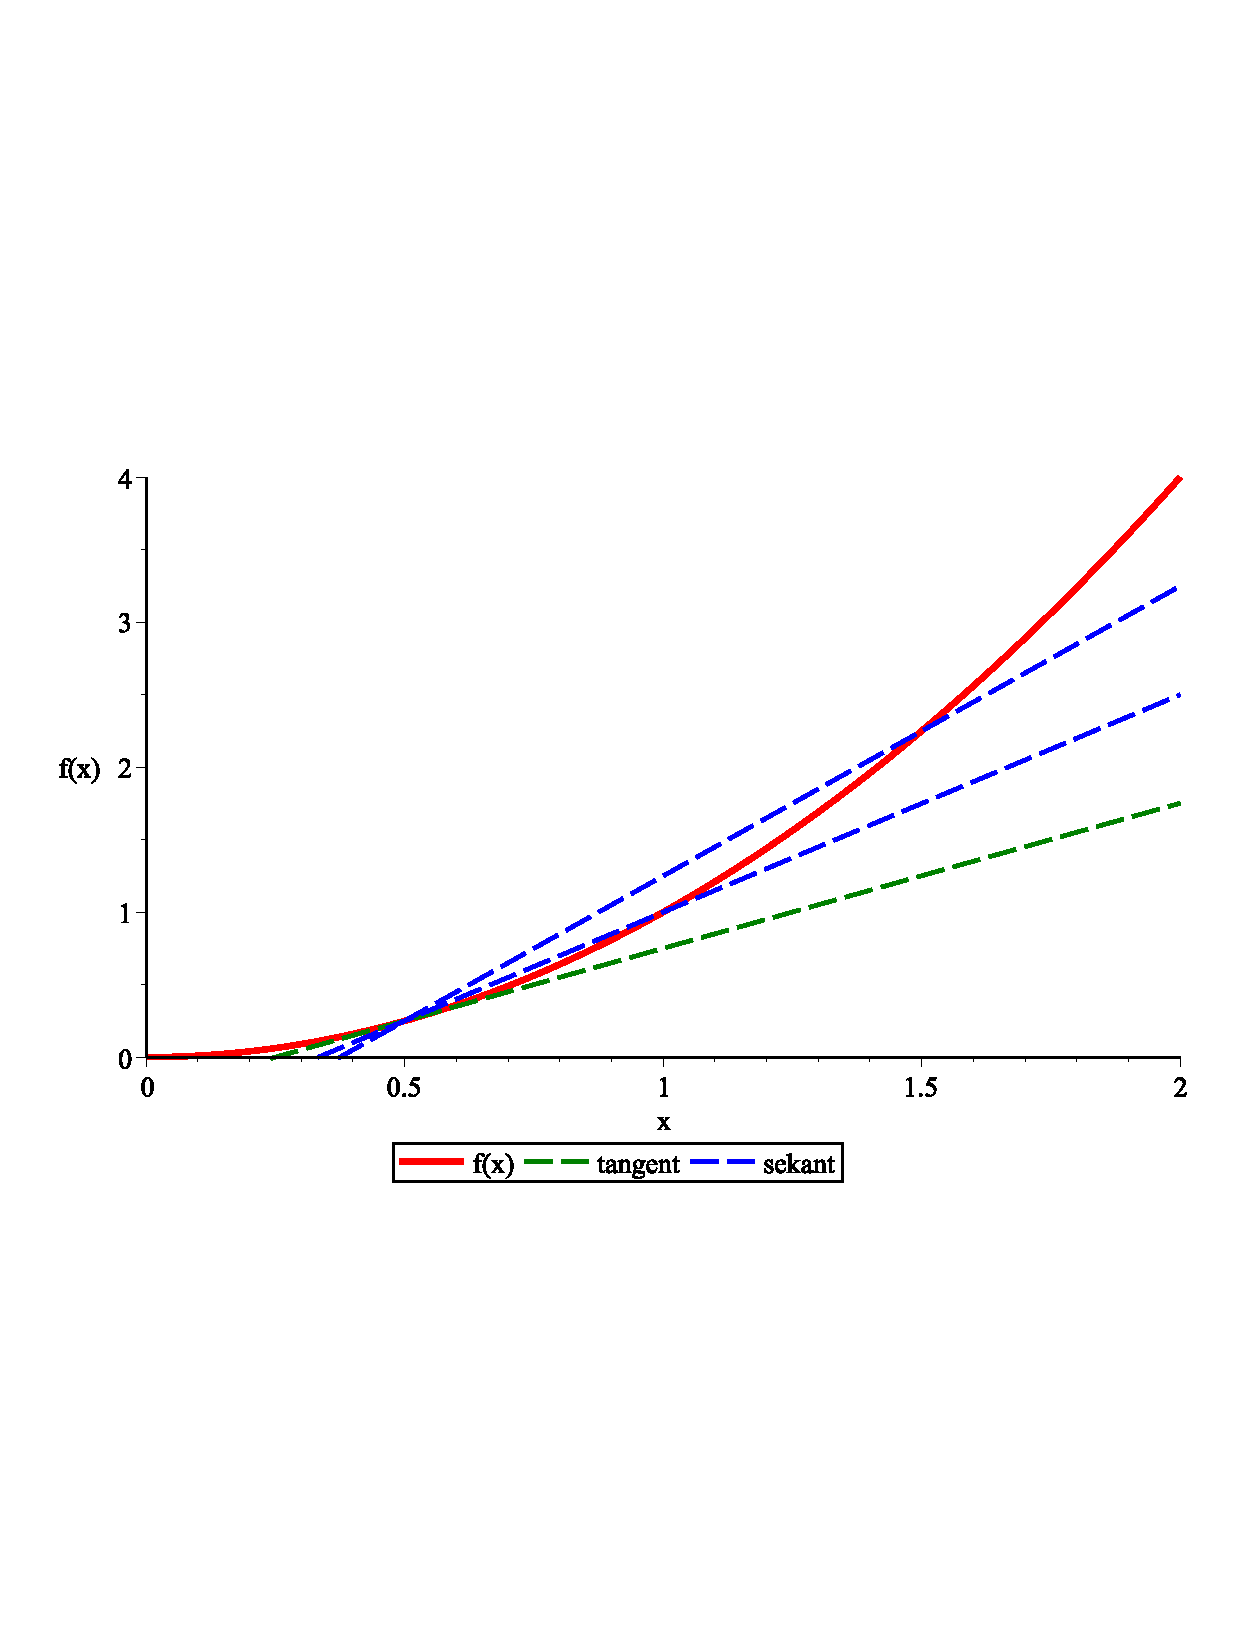
\includegraphics[width=0.8\textwidth, clip, trim=0 7.8cm 0 6cm]{secant}
	\caption{Afbildning af $f(x)=x^2$ med en tangent i punktet $x=0.5$ (grøn) og to sekantlinier (blå) med $h=0.5, 1.0$. Hældningen af sekantlinierne ses at gå mod hældningen af tangentlinien når $h$ bliver mindre.}
	\label{fig:secanttangent}
\end{figure}

\subsection{Den aflede som funktion}
Den funktion som sender alle punkter $a$ over i den afledte af $f(x)$ i punktet $a$. Denne funktion kaldes \emph{den aflede funktion} af $f(x)$ og skrives som $\frac{df}{dx}$ i Leibnizs notation ($f'(x)$ i Lagranges notation).

Den aflede funktion kan bestemmes ud fra ligning \eqref{eq:diffcoef}. Tag for eksempel den aflede funktion af en potensfunktion $f(x) = x^n$ med $n \in \mathbb{N}$ og $n \geq 1$:
\begin{align}
\frac{d}{dx}x^n =& \lim_{h\to0}\frac{f(x+h) - x^n}{h} \\
                =& \lim_{h\to0}\frac{(x+h)^n - x^n}{h}\label{eq:powerstuck}
\end{align}
Her har vi brug for at huske faktoriseringen af $a^n - b^n$:
\begin{equation}
a^n - b^n = (a-b)(a^{n-1} + a^{n-2}b + a^{n-3}b^2 + \cdots + a b^{n-2} + b^{n-1})
\end{equation} 
Hvis vi sætter $a=x+h$ og $b=x$, hvilket betyder at $a-b=x+h-x=h$, kan vi komme videre:
\begin{align}
\frac{d}{dx}x^n &= \lim_{h\to0}\frac{h((x+h)^{n-1} + (x+h)^{n-2}x + \cdots + (x+h)x^{n-2} + x^{n-1})}{h}\notag \\
                &= \lim_{h\to0}\left(\underbrace{(x+h)^{n-1} + (x+h)^{n-2}x + \cdots + (x+h)x^{n-2} + x^{n-1}}_
                   {n\text{ led som alle giver } x^{n-1}\text{ for } h\to0}\right)\notag \\
\frac{d}{dx}x^n &= nx^{n-1}\label{eq:generalpowerfunc}
\end{align}
Ligning \eqref{eq:generalpowerfunc} kan udvides til at gælle negative eksponenter og rationelle eksponenter vha. andre differentiationsregneregler.

\section{Integration}
Integration er det andet store emne i calculus og det inverse af differentiation. 
\subsection{Bestemte integraler}

\subsection{Ubestemt integraler}
\end{document}